\documentclass[11pt, a4paper]{article}
%\usepackage{proj1}
\usepackage{natbib}
\usepackage{fancyhdr}  
\usepackage{subcaption}
\usepackage{caption}
\usepackage{graphicx}
\usepackage{numprint}
\usepackage{multirow}
\linespread{1.25} 
\setlength{\parindent}{0cm}
\graphicspath{{Images/}}
\usepackage{hyperref}
\usepackage{amsmath}
\usepackage{amsfonts}
\usepackage{amssymb}
\usepackage{amsthm}
\usepackage{mathtools}
\usepackage{commath}
\usepackage{bbm}

%\usepackage[sc,osf]{mathpazo}
\usepackage{subcaption}
\usepackage[a4paper, top=1in, left=1.0in, right=1.0in, bottom=1in, includehead, includefoot]{geometry} %Usually have top as 1in

\usepackage{listings}
\usepackage{color} %red, green, blue, yellow, cyan, magenta, black, white
\definecolor{mygreen}{RGB}{28,172,0} % color values Red, Green, Blue
\definecolor{mylilas}{RGB}{170,55,241}


\hypersetup{colorlinks,linkcolor={black},citecolor={blue},urlcolor={black}}
\usepackage{color}
\urlstyle{same}


\theoremstyle{definition}
\newtheorem{definition}{Definition}[section]

%\newcommand{\Sta}{\rho}
\newcommand{\adja}{q_a}
\newcommand{\adjb}{q_b}
\newcommand{\adjaB}{q_{a,\partial \Omega}}
\newcommand{\adjbB}{q_{b,\partial \Omega}}
%\newcommand{\Con}{u}
\newcommand{\ra}{\rho_a}
\newcommand{\rb}{\rho_b}
\newcommand{\w}{\mathbf{w}}
\newcommand{\Stav}{\mathbf{v}}
\newcommand{\Adja}{\mathbf{p}}
\newcommand{\Adjb}{q}
\newcommand{\Adjc}{{p}_{\partial \Sigma}}
\newcommand{\Con}{\mathbf{f}}
\newcommand{\n}{\mathbf{n}}
\newcommand{\h}{\mathbf{h}}
\newcommand{\K}{\mathbf{K}}


\pagenumbering{gobble}
\begin{document}
	\section*{Report 03/12/2020}
	
	\section{Time independent control}
	We have the following OCP:
	\begin{align*}
		&J = \frac{1}{2}\int_0^T \int_\Omega (\rho - \widehat \rho)^2 dr dt + \frac{\beta}{2} \int_\Omega \w(r)^2 dr\\
		&\text{subject to:}\\
		&\frac{\partial \rho}{\partial t} = \nabla^2 \rho - \nabla \cdot (\rho \w(r))
	\end{align*}
	Then the Lagrangian is:
	\begin{align*}
		\mathcal{L}(\rho,\w, q) &=  \frac{1}{2}\int_0^T \int_\Omega (\rho - \widehat \rho)^2 dr dt + \frac{\beta}{2} \int_\Omega \w(r)^2 dr \\
		&- \int_0^T \int_\Omega q\frac{\partial \rho}{\partial t} - q\nabla^2 \rho + q\nabla \cdot (\rho \w) dr dt.
	\end{align*}
	And after integrating by parts (neglecting the BCs because we know them already):
	\begin{align*}
		\mathcal{L}(\rho,\w, q) &=  \frac{1}{2}\int_0^T \int_\Omega (\rho - \widehat \rho)^2 dr dt + \frac{\beta}{2} \int_\Omega \w(r)^2 dr \\
		&- \int_0^T \int_\Omega q\frac{\partial \rho}{\partial t} - q\nabla^2 \rho -  \rho \w \cdot \nabla q dr dt.
	\end{align*}
	Taking derivatives with respect to $\w$ gives:
	\begin{align*}
		\mathcal{L}(\rho,\w, q) &= \int_\Omega \beta \w(r) \cdot \h(r) dt + \int_0^T \int_\Omega \rho \h(r) \cdot \nabla q dr dt.
	\end{align*}
	Since $\w$ does not depend on $t$, neither does $\h$ and so this can be taken out of the time integral:
	\begin{align*}
		\mathcal{L}(\rho,\w, q) &= \int_\Omega \bigg( \beta \w(r) \cdot \h(r)  + \h(r) \cdot \int_0^T \rho  \nabla q dt \bigg) dr.
	\end{align*}
	Then we get:
	\begin{align*}
		\beta \w(r)  +  \int_0^T \rho  \nabla q dt = 0
	\end{align*}
	And finally:
	\begin{align*}
		\w(r) = - \frac{1}{\beta} \int_0^T \rho  \nabla q dt
	\end{align*}
	
	\section{$V_{ext}$ control}
	We have the following OCP:
	\begin{align*}
		&J = \frac{1}{2}\int_0^T \int_\Omega (\rho - \widehat \rho)^2 dr dt + \frac{\beta}{2} \int_0^T\int_\Omega V_{ext}^2 dr\\
		&\text{subject to:}\\
		&\frac{\partial \rho}{\partial t} = \nabla^2 \rho + \nabla \cdot (\rho \nabla V_{ext})
	\end{align*}
	The Lagrangian is:
	\begin{align*}
		\mathcal{L}(\rho, V_{ext}, q) &= \frac{1}{2}\int_0^T \int_\Omega (\rho - \widehat \rho)^2 dr dt + \frac{\beta}{2} \int_0^T\int_\Omega V_{ext}^2 dr\\
		&- \int_0^T \int_\Omega q\frac{\partial \rho}{\partial t} - q\nabla^2 \rho - q\nabla \cdot (\rho \nabla V_{ext}) dr dt.
	\end{align*}
	We need to integrate by parts twice to get the term in $V_{ext}$ into the necessary form:
	\begin{align*}
		\int_0^T \int_\Omega q \nabla \cdot (\rho \nabla V_{ext}) dr dt &= \int_0^T \int_{\partial \Omega} q \rho \nabla V_{ext} \cdot \n dr dt - \int_0^T \int_\Omega \rho \nabla V_{ext} \cdot \nabla q dr dt \\
		& = \int_0^T \int_{\partial \Omega} q \rho \nabla V_{ext} \cdot \n  - \rho V_{ext} \nabla q \cdot \n dr dt + \int_0^T \int_\Omega V_{ext} \nabla \cdot (\rho \nabla q) dr dt
	\end{align*}
	We will also have 
	\begin{align*}
		\int_0^T \int_\Omega q\nabla^2 \rho = \int_0^T \int_{\partial \Omega} q \nabla \rho \cdot \n- \rho \nabla q \cdot \n dr dt + \int_0^T \int_\Omega \rho \nabla^2 q dr dt
	\end{align*}
	\subsection{Boundary Conditions}
	And the boundary conditions:
	\begin{align*}
		\int_0^T \int_{\partial \Omega} q_{\partial \Omega}\nabla \rho \cdot \n + q_{\partial \Omega}\rho \nabla V_{ext} \cdot \n dr dt
	\end{align*}
	Combining these:
	\begin{align*}
		&\int_0^T \int_{\partial \Omega} q \rho \nabla V_{ext} \cdot \n  - \rho V_{ext} \nabla q \cdot \n + q \nabla \rho \cdot \n - \rho \nabla q \cdot \n + q_{\partial \Omega}\nabla \rho \cdot \n + q_{\partial \Omega}\rho \nabla V_{ext} \cdot \n dr dt
	\end{align*}
	During the derivation of the adjoint equation we have:

	\begin{align*}
		\int_0^T \int_{\partial \Omega} \n \cdot h \bigg(q  \nabla V_{ext} -  V_{ext} \nabla q -\nabla q + q_{\partial \Omega} \nabla V_{ext} \bigg) +
		\nabla h \cdot \n \bigg(q  + q_{\partial \Omega}  \bigg)dr dt
	\end{align*}
Then from the $\nabla h$ terms we get $q_{\partial \Omega} = - q$ and so:
\begin{align*}
	(q  \nabla V_{ext} -  V_{ext} \nabla q -\nabla q - q \nabla V_{ext}  ) \cdot \n = 0
\end{align*}
	And therefore:
	\begin{align*}
		(1 + V_{ext})\frac{\partial q}{\partial n} = 0
	\end{align*}
Can we divide by $1 + V_{ext}$, is $V_{ext} > 0$.
	\subsection{Gradient Equation}
	We take the derivative of the Lagrangian with respect to $V_{ext}$:
	\begin{align*}
		\mathcal{L}_{V_{ext}} (\rho, V_{ext},q)h &= \int_0^T \int_\Omega \beta V_{ext} h + \nabla \cdot (\rho \nabla q) h dr dt \\
		&+\int_0^T \int_{\partial \Omega} (q \rho \nabla h - \rho h \nabla q - q \rho \nabla h) \cdot \n dr dt
	\end{align*}
	The boundary conditions just give (as before) $\frac{\partial q}{\partial n} = 0$ since $\rho >0$. (+++ We don't do this, do we? But it would support my hypothesis that $1 + V_{ext}) >0$ +++)
	Then from the terms within the domain we have:
	\begin{align*}
		\beta V_{ext}  + \nabla \cdot (\rho \nabla q)  = 0
	\end{align*}
	And finally 
	\begin{align*}
		V_{ext} = - \frac{1}{\beta} \nabla \cdot (\rho \nabla q).
	\end{align*}
	
	
	\section{Target at final time}
	
		\begin{align*}
		&J = \frac{1}{2} \int_\Omega (\rho(T) - \widehat \rho)^2 dr  + \frac{\beta}{2} \int_0^T\int_\Omega \w^2 dr\\
		&\text{subject to:}\\
		&\frac{\partial \rho}{\partial t} = \nabla^2 \rho - \nabla \cdot (\rho \w)
	\end{align*}
	Then the Lagrangian is:
	\begin{align*}
		\mathcal{L}(\rho,\w, q) &= \frac{1}{2} \int_\Omega (\rho(T) - \widehat \rho)^2 dr  + \frac{\beta}{2} \int_0^T\int_\Omega \w^2 dr\\
		&- \int_0^T \int_\Omega q\frac{\partial \rho}{\partial t} - q\nabla^2 \rho + q\nabla \cdot (\rho \w) dr dt.
	\end{align*}
	From integrating by parts we get:
	\begin{align*}
	\int_0^T \int_\Omega	-q\frac{\partial \rho}{\partial t} dr dt= - \int_\Omega q(T) \rho(T) - q(0) \rho(0) dr +  \int_0^T \int_\Omega	\rho \frac{\partial q}{\partial t} dr dt
	\end{align*}
		\begin{align*}
		\mathcal{L}(\rho,\w, q) &= \frac{1}{2} \int_\Omega (\rho(T) - \widehat \rho)^2 dr  + \frac{\beta}{2} \int_0^T\int_\Omega \w^2 dr\\
		&- \int_\Omega q(T) \rho(T) - q(0) \rho(0) dr + \int_0^T \int_\Omega \rho \frac{\partial q}{\partial t}   + q\nabla^2 \rho - q\nabla \cdot (\rho \w) dr dt.
	\end{align*}
	Taking the derivative with respect to $\rho $ gives:
	\begin{align*}
		\mathcal{L}_\rho(\rho,\w, q)h &= \int_\Omega  (\rho(T) - \widehat \rho) h(T) dr - \int_\Omega q(T) h(T) dr\\
		&+ \int_0^T \int_\Omega h \frac{\partial q}{\partial t}   + q\nabla^2 h - q\nabla \cdot (h \w) dr dt.
	\end{align*}
	Considering the terms for $h(T)$ gives:
	\begin{align*}
		(\rho(T) - \widehat \rho) - q(T) = 0,
	\end{align*}
	and so 
	\begin{align*}
	q(T) = \rho(T) - \widehat \rho
	\end{align*}
	The adjoint PDE remains unchanged, except for the fact that $ \rho - \widehat \rho$ does not enter the PDE anymore.

	\section{Sedimentation}
	I ran the two different configurations with N = 100. I computed the mass in both cases and plotted the outcome. We can see that mass is still not constant but it is better than with $ N = 70$. 
	
	\begin{figure}[h]
		\centering
		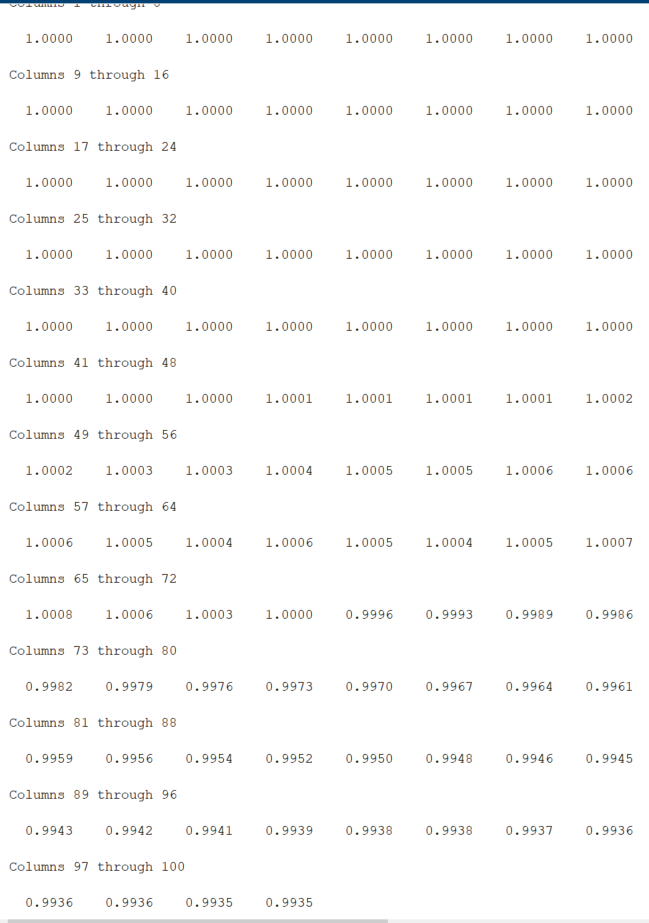
\includegraphics[scale=0.6]{rhobar0072.png}
		\caption{Figure 8 in paper, mass for each time} 
		\label{F1}
	\end{figure}
	\begin{figure}[h]
		\centering
		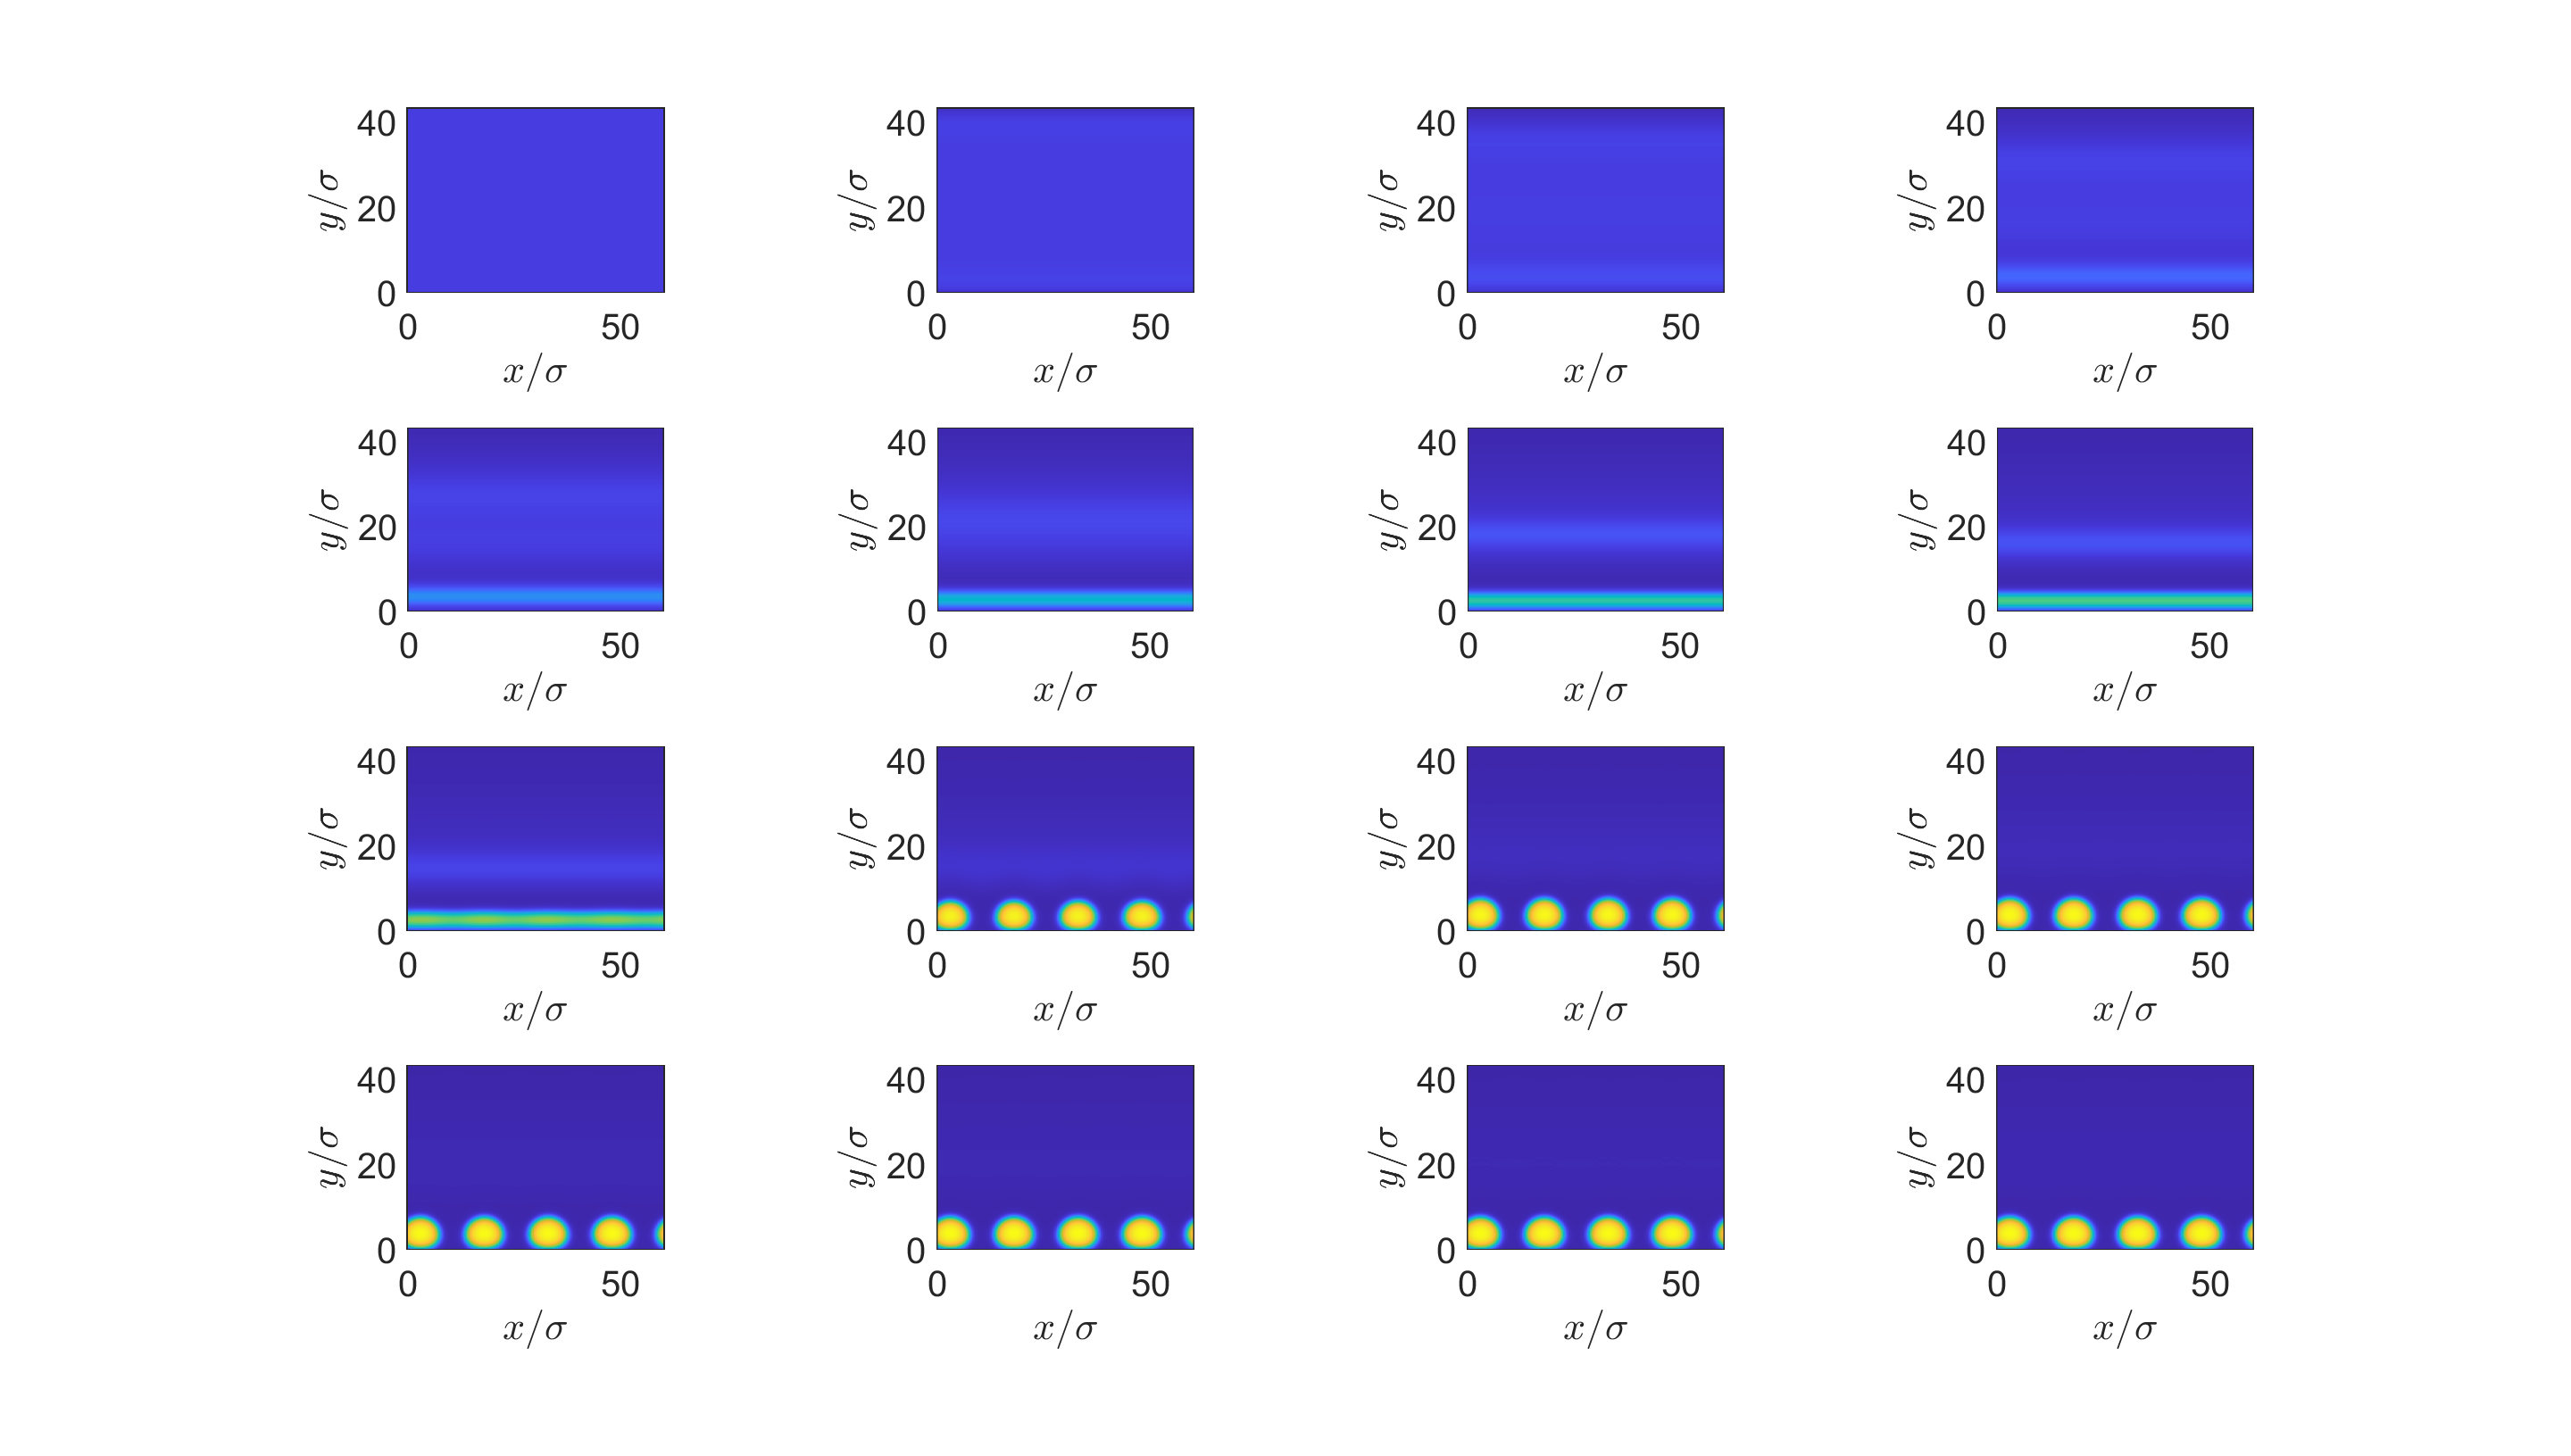
\includegraphics[scale=0.25]{Plotrhobar0072.png}
		\caption{Figure 8 in paper, result at each time} 
		\label{F2}
	\end{figure}
	\begin{figure}[h]
		\centering
		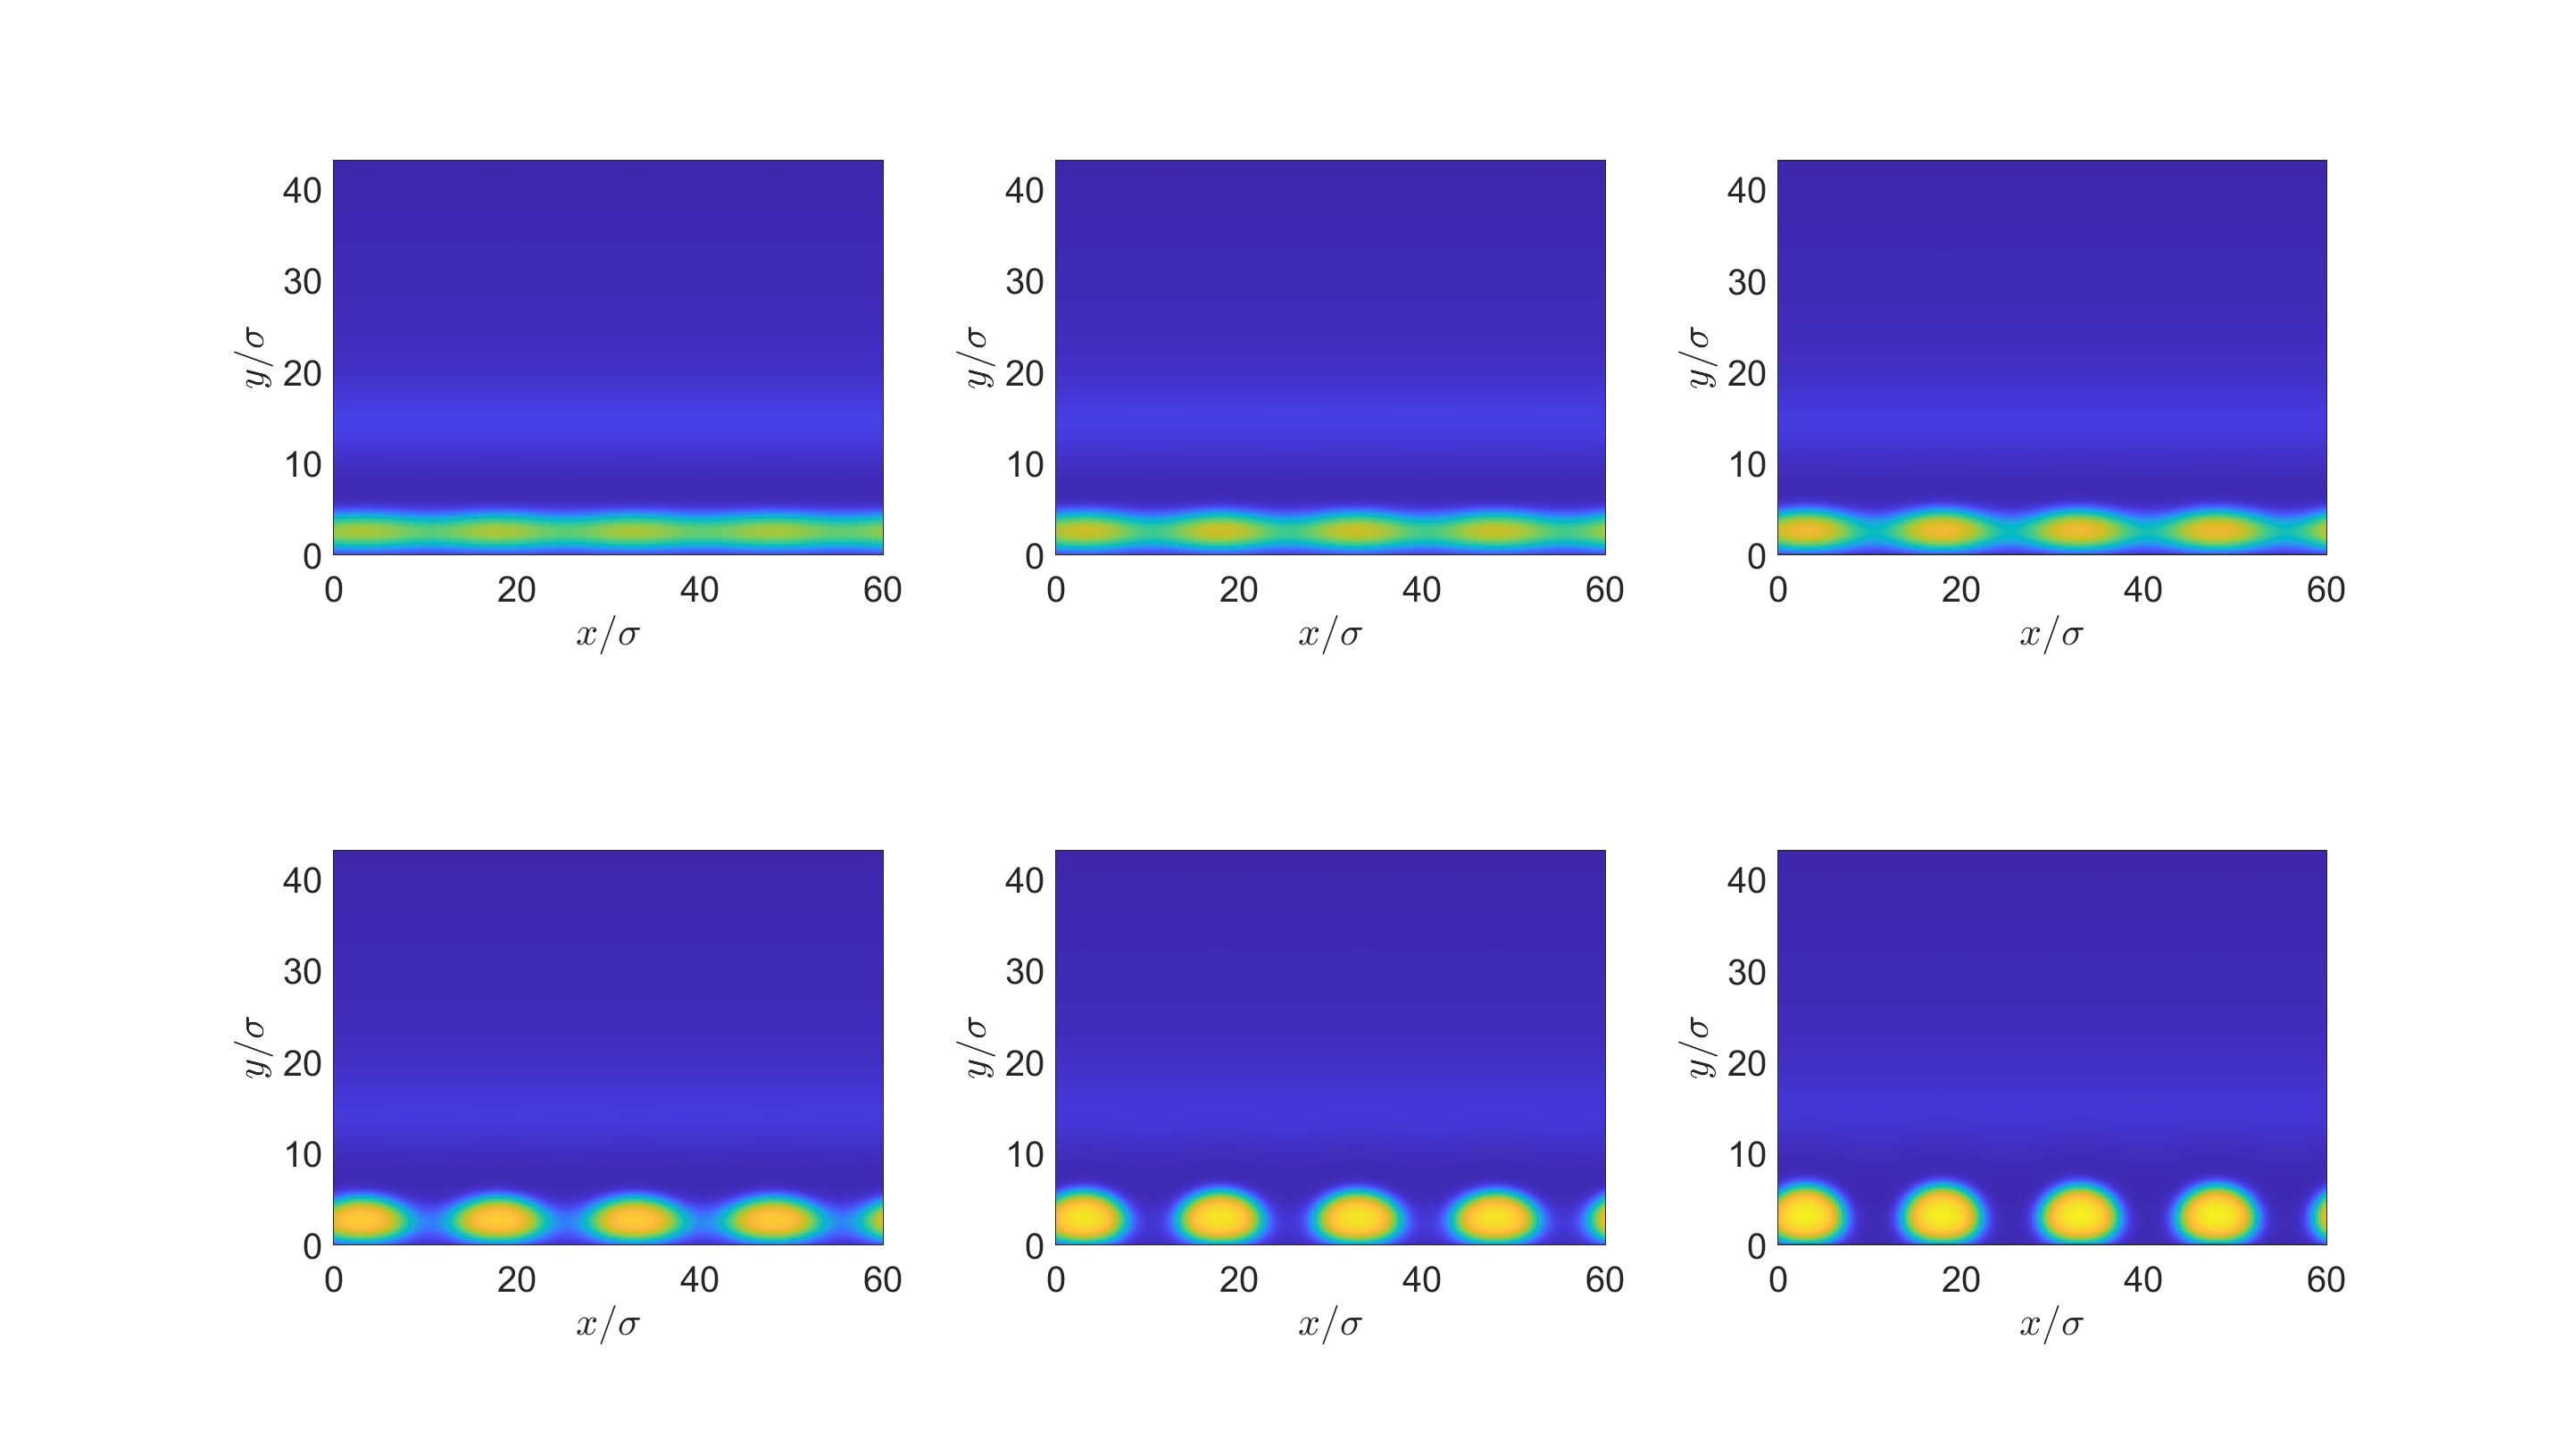
\includegraphics[scale=0.25]{rhobar0072Zoom57to62.png}
		\caption{Figure 8 in paper, result at times 57 - 62 out of 100} 
		\label{F3}
	\end{figure}
		\begin{figure}[h]
		\centering
		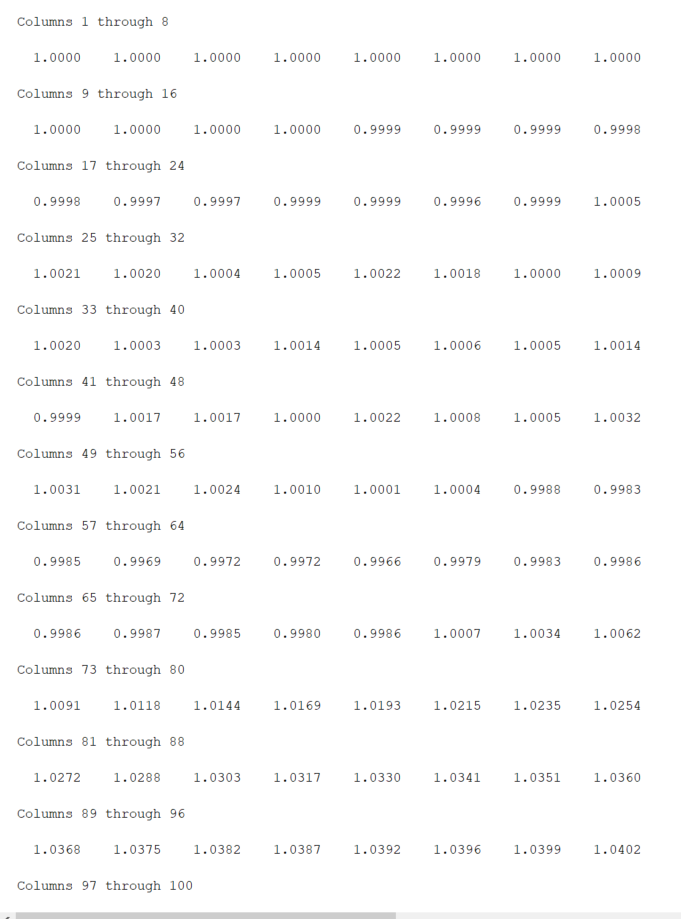
\includegraphics[scale=0.6]{rhobar02.png}
		\caption{Figure 10 in paper, mass for each time} 
		\label{F4}
	\end{figure}
	\begin{figure}[h]
		\centering
		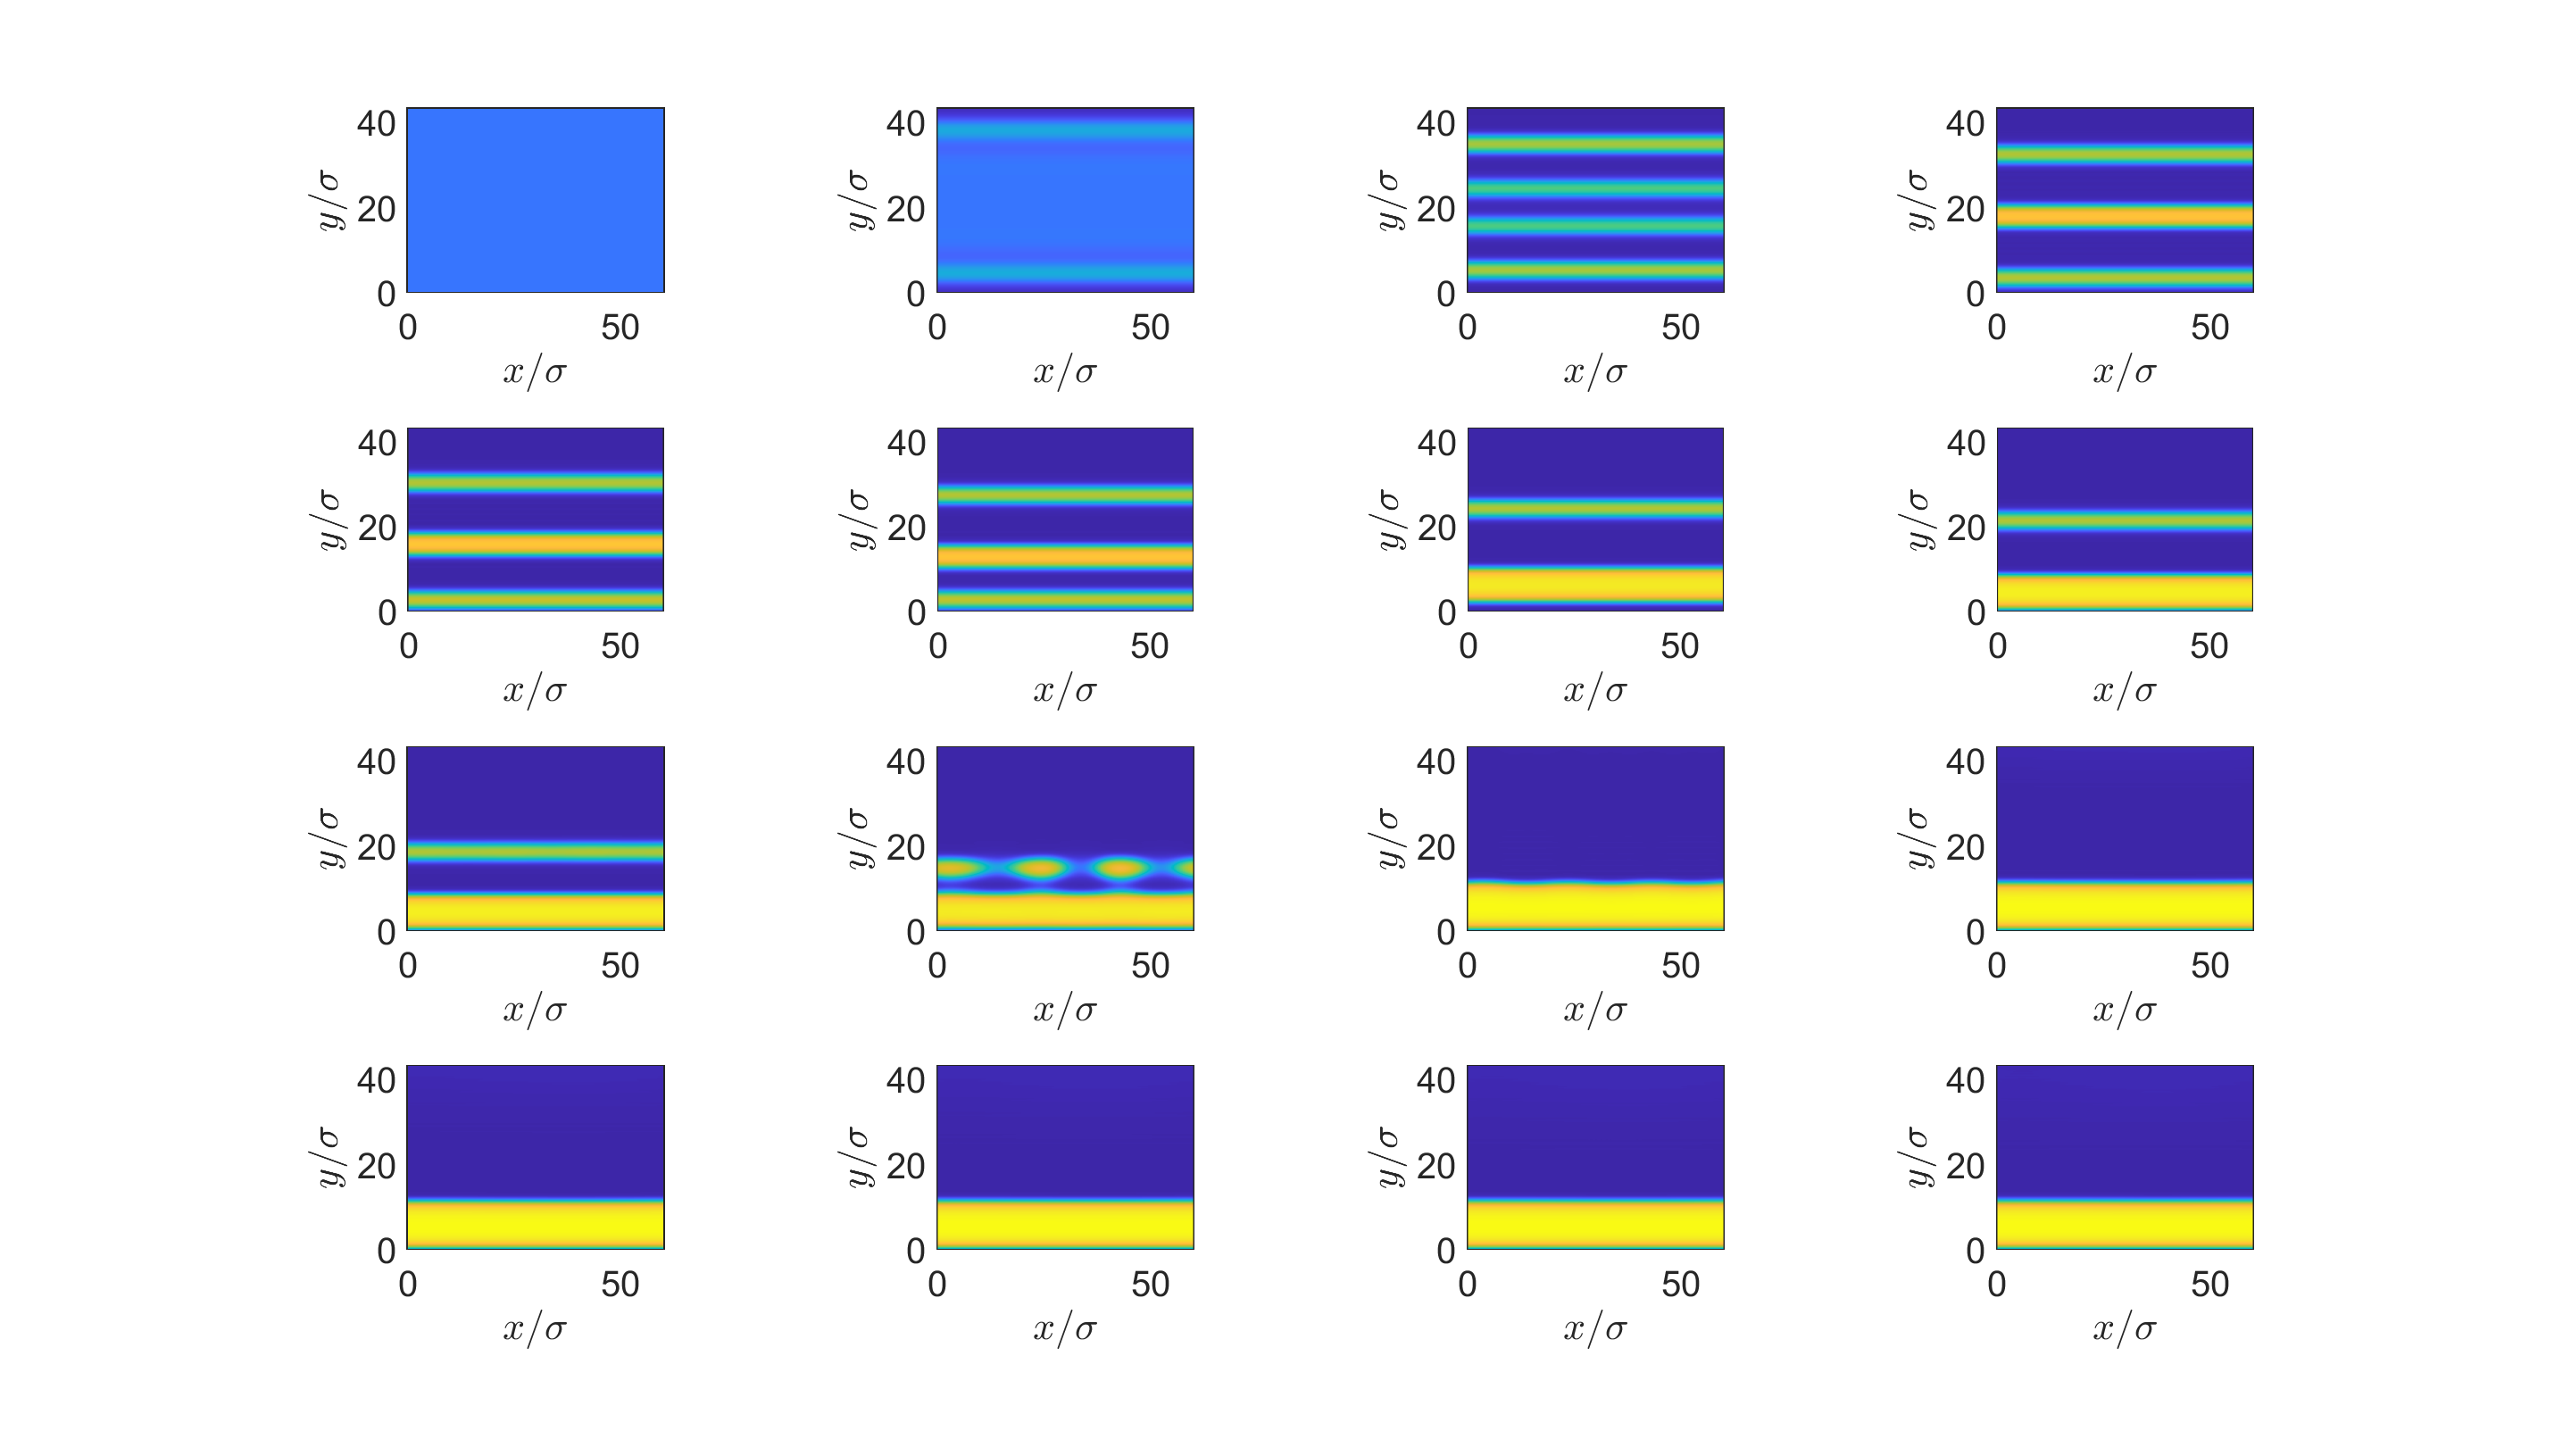
\includegraphics[scale=0.25]{Plotrhobar02.png}
		\caption{Figure 10 in paper, result at each time} 
		\label{F5}
	\end{figure}
	\begin{figure}[h]
		\centering
		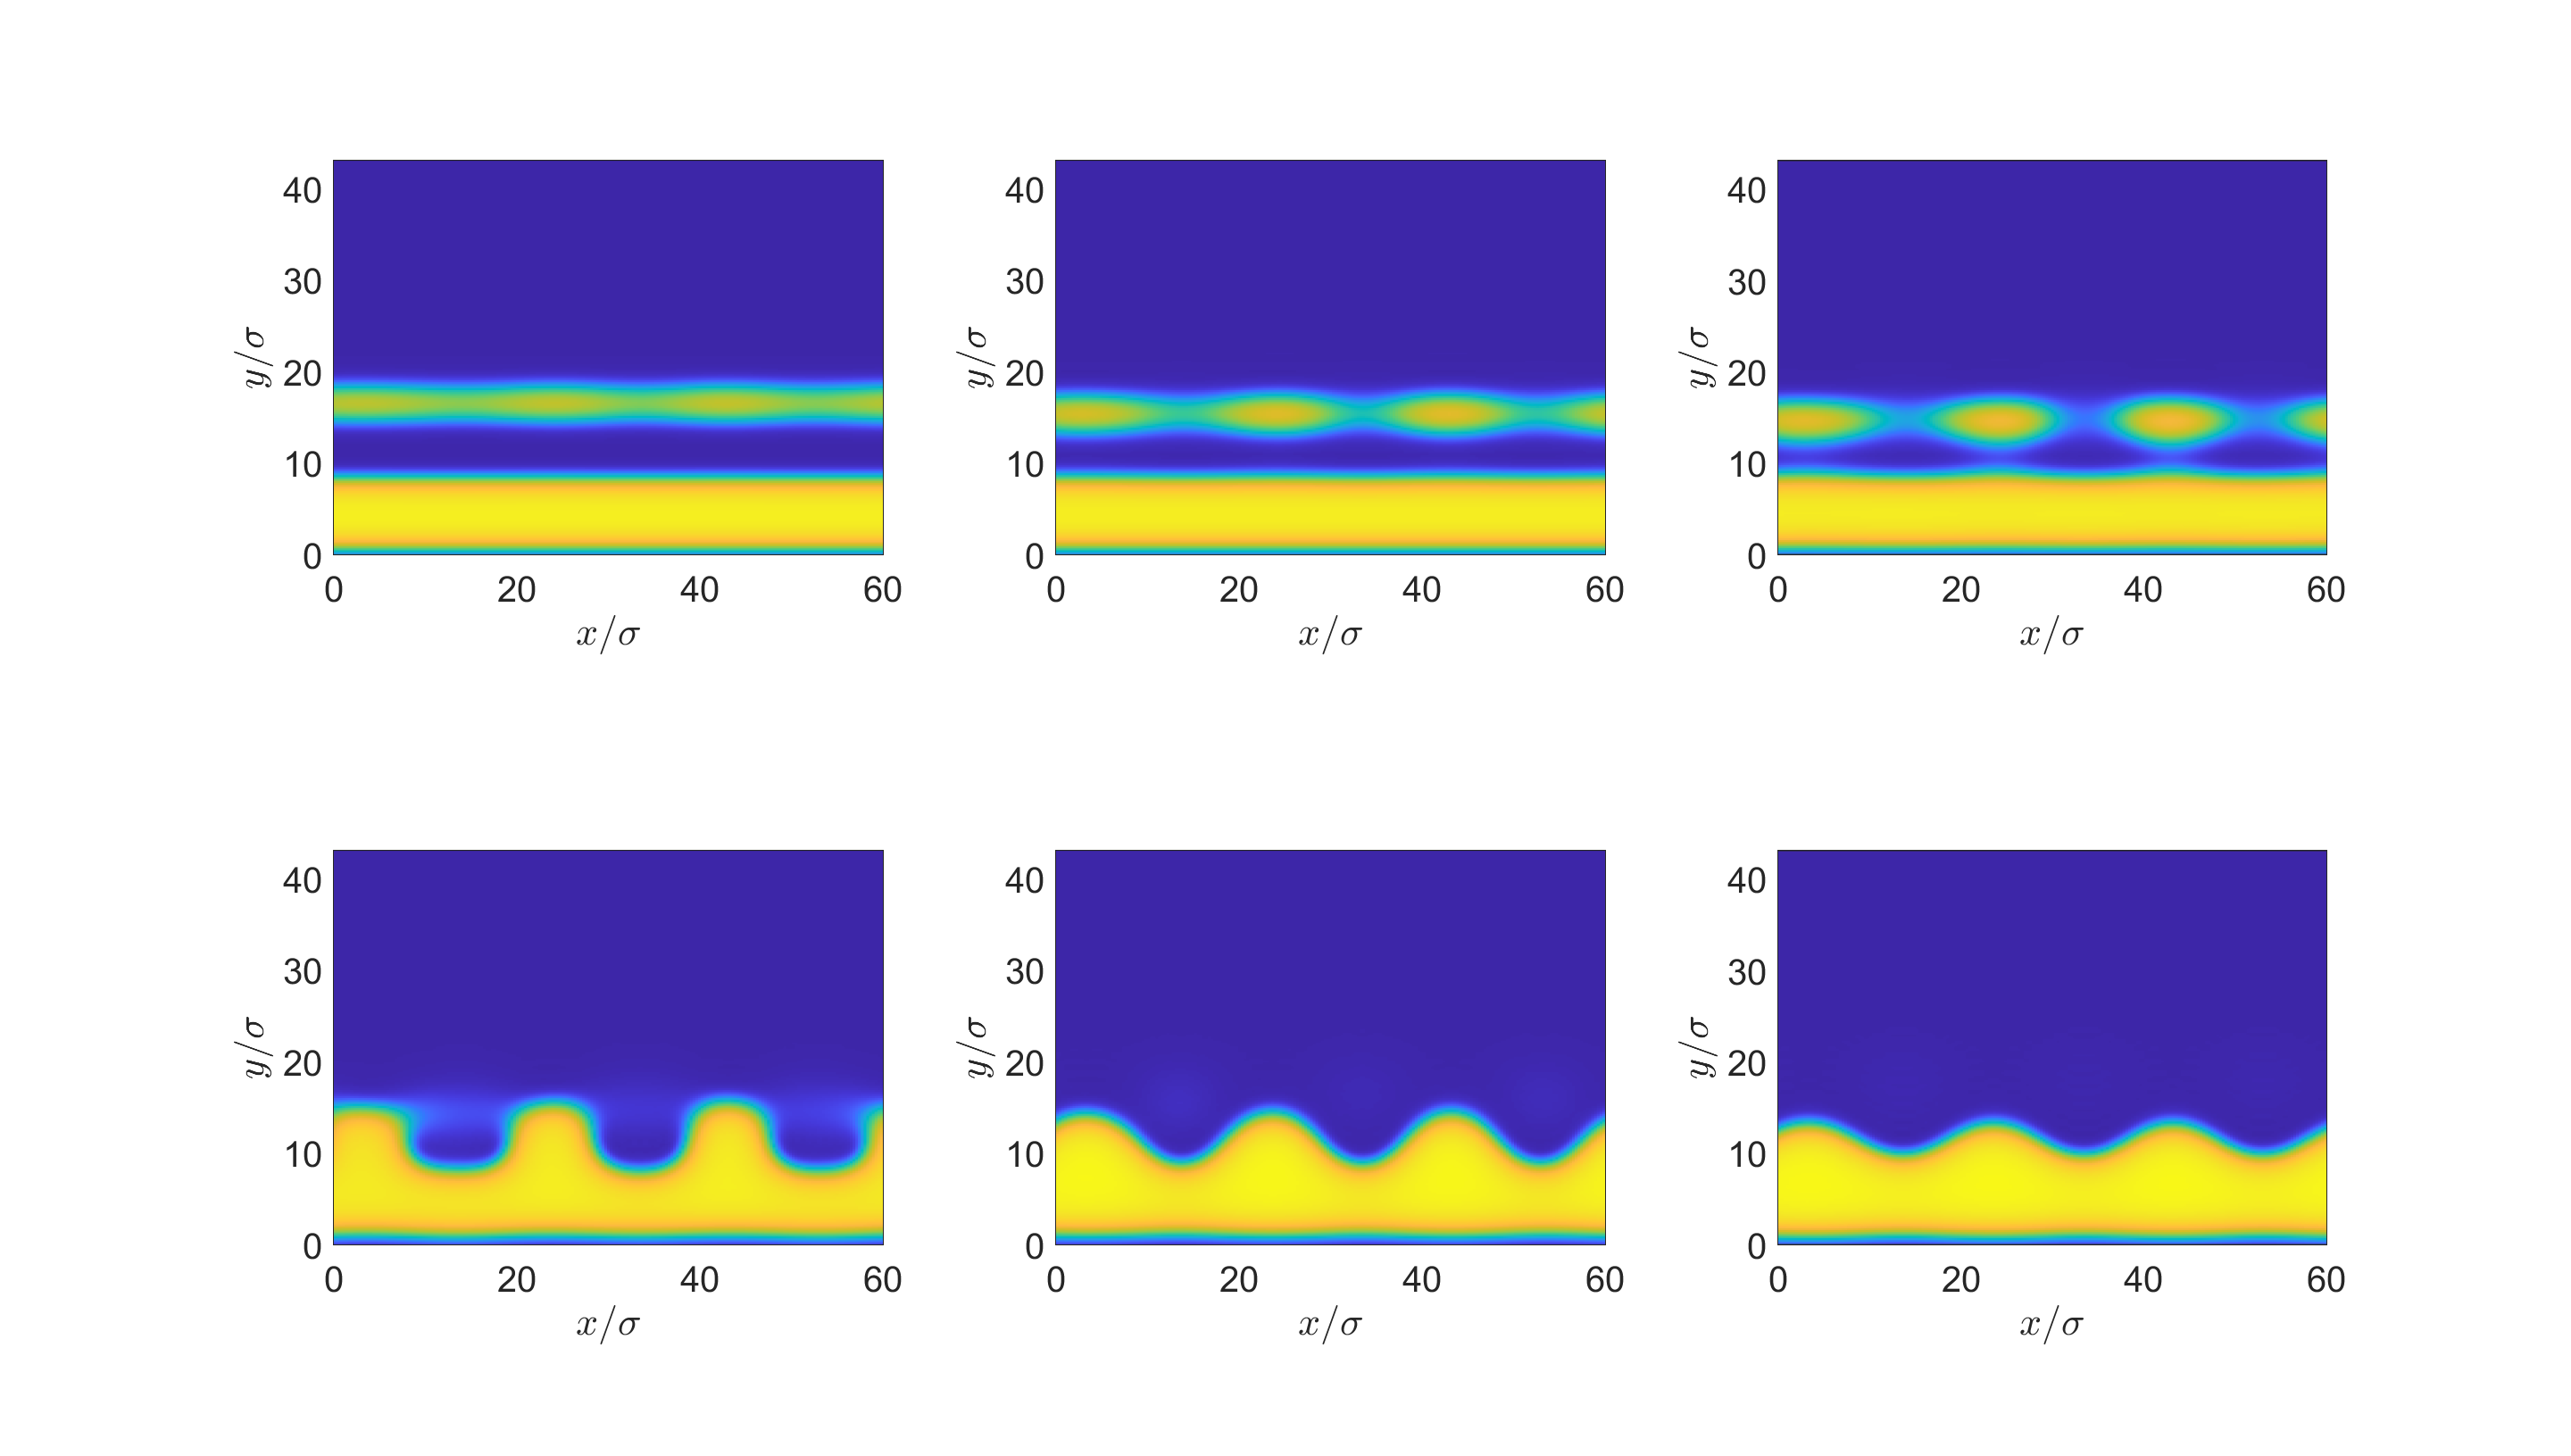
\includegraphics[scale=0.25]{rhobar02Zoom60to66.png}
		\caption{Figure 8 in paper, result at times 60 - 66 out of 100} 
		\label{F6}
	\end{figure}
	
\section{MultipleSpecies forward problem}
	The forward problem is showing weird oscillations. Maybe I implemented this incorrectly. Figure \ref{F7} shows what happens with diffusion only. Figure \ref{F8} and \ref{F9} shows what happens with advection in opposite direction, attraction to the own species and repulsion with the other
	\begin{figure}[h]
		\centering
		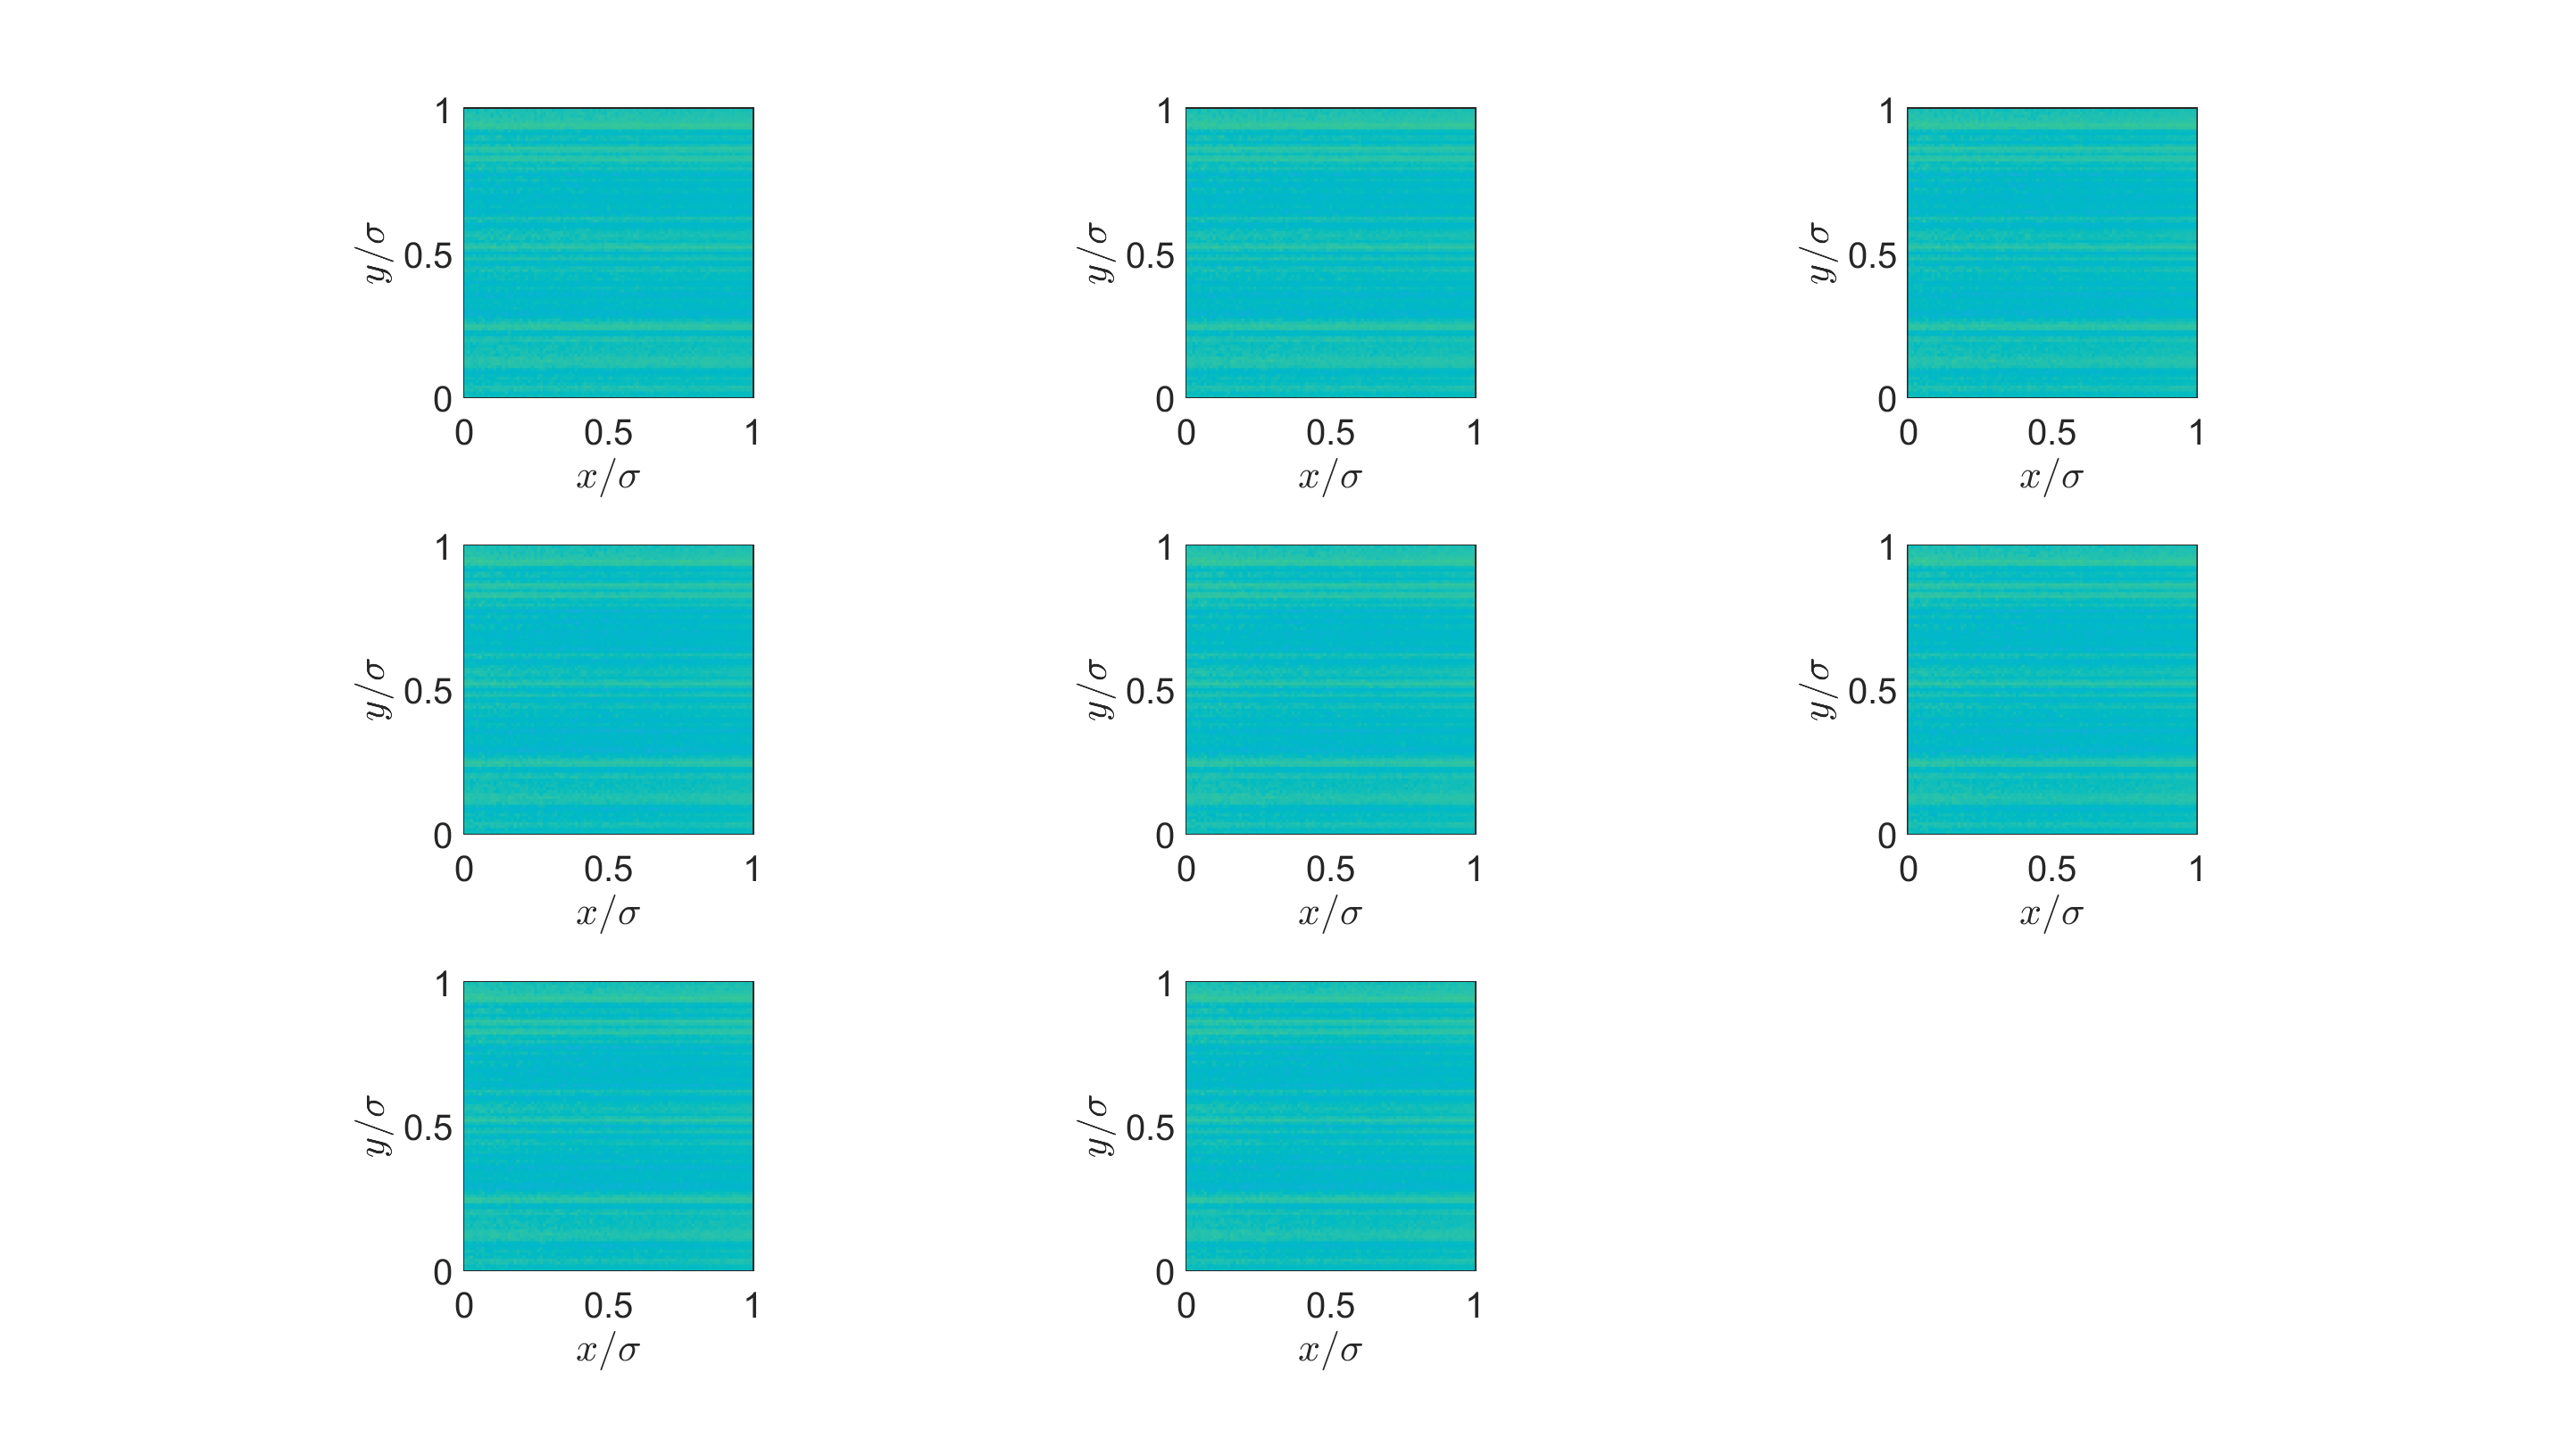
\includegraphics[scale=0.25]{Weird.png}
		\caption{Weird Oscillations for diffusion only} 
		\label{F7}
	\end{figure}
	\begin{figure}[h]
		\centering
		\includegraphics[scale=0.25]{Cool1.png}
		\caption{Maybe plausible behaviour $\rho_a$} 
		\label{F8}
	\end{figure}
\begin{figure}[h]
	\centering
	\includegraphics[scale=0.25]{Cool2.png}
	\caption{Maybe plausible behaviour $\rho_b$} 
	\label{F9}
\end{figure}

\section{Other}
- sedimentation optimality conditions
- next week
- holiday

\end{document}